\chapter{既存手法}
\label{chap:related_works}

\section{Java仮想マシン}

ハードウェアやオペレーティングシステムといったプラットフォームが異なる環境下で同一の実行形式を利用する方法として、
プログラムをプラットフォームに独立な中間表現で記述し、各プラットフォーム向けに実装された仮想マシン上で実行する、という手法がある。

Java仮想マシン(Java Virtual Machine, JVM)\cite{jvms}は、広く用いられている仮想マシンの一つである。
JVMは、プログラミング言語Javaの前身であるOakのための仮想マシンとして、James Goslingらによって設計された。

\subsection{classファイル}

JVMでは、プログラムはクラス単位で\verb|class|ファイルと呼ばれる実行形式にコンパイルされる。
\verb|class|ファイルの構成を\ref{fig:jvm_class_file}に示す。

\begin{figure}[htbp]
  \caption{classファイル概観}
  \label{fig:jvm_class_file}
  \begin{center}
    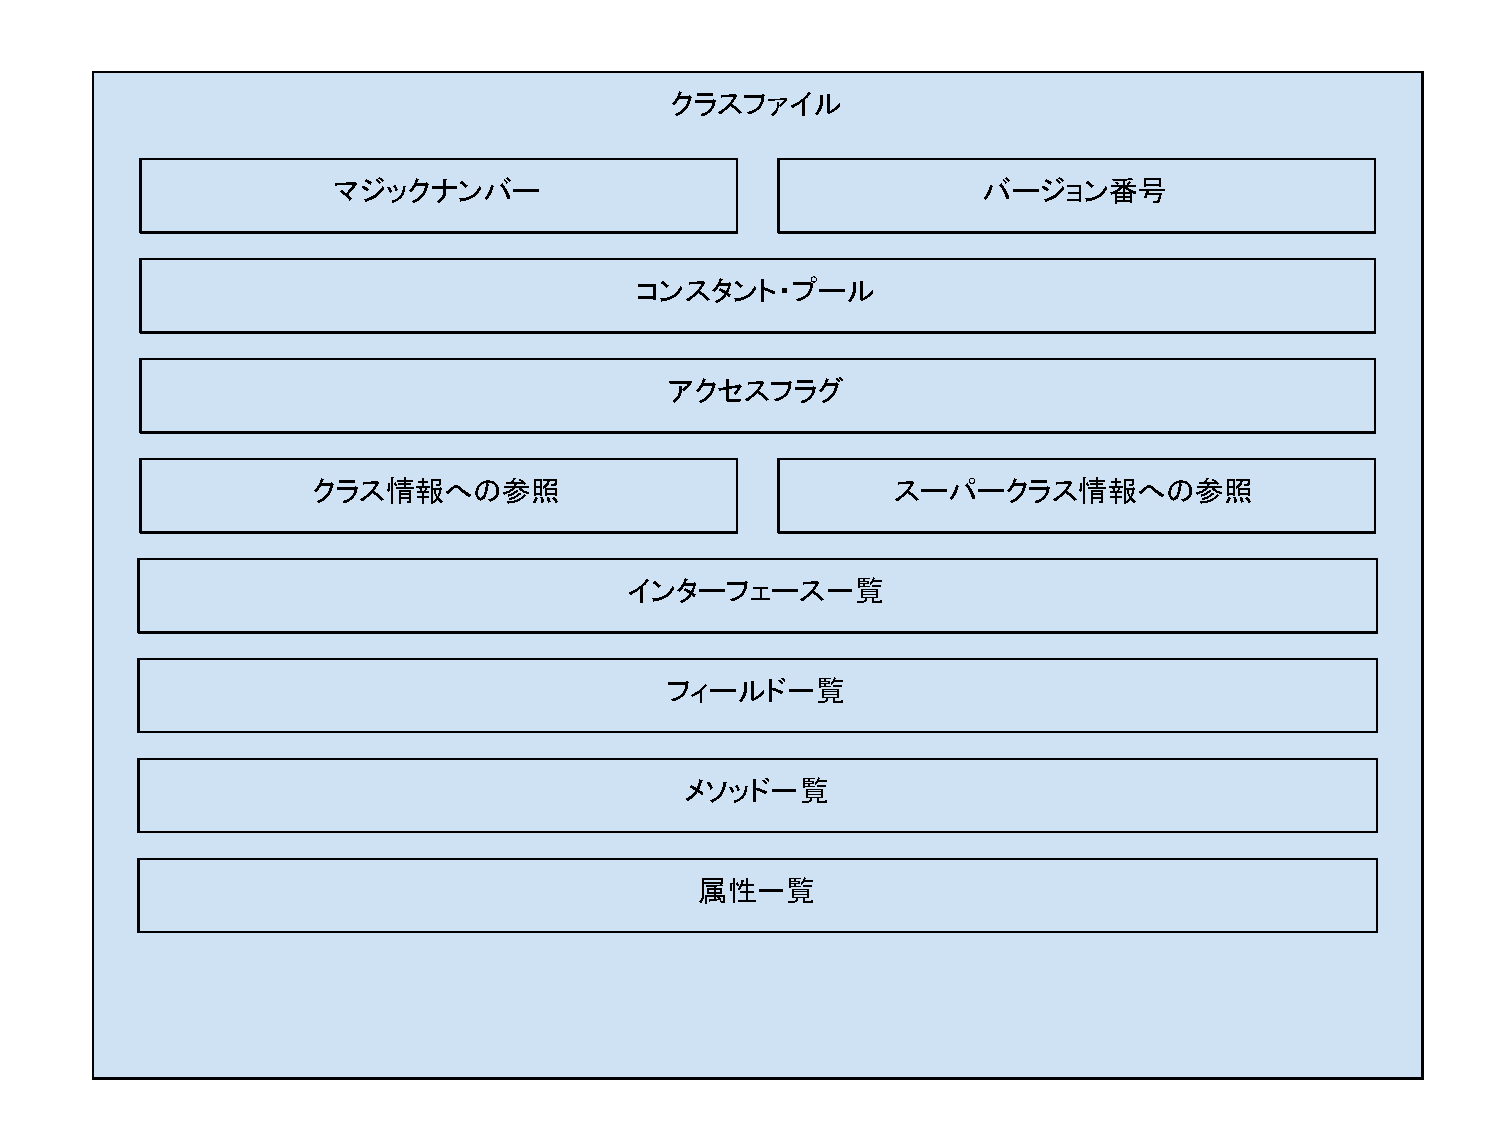
\includegraphics[bb=0 0 800 600,width=12cm]{img/jvm_class_file.pdf}
  \end{center}
\end{figure}

\verb|class|ファイルは、マジックナンバー(\verb|0xCAFEBABE|)と、\verb|class|ファイルのフォーマットのバージョンを表す計4バイトの番号情報を持つ。

コンスタント・プールには、この\verb|class|ファイル内で参照される静的な文字列、クラス名、インターフェース名、フィールド名、メソッド名等の定数が格納されている。

アクセスフラグは、この\verb|class|ファイルがクラスまたはインターフェースのどちらを定義したものか、定義されたクラスまたはインターフェースが外部からアクセス可能か、といった属性を表す。

\verb|class|ファイルは、その\verb|class|ファイルによって定義されるクラスまたはインターフェースを表す情報を指し示すコンスタント・プールへの参照を持つ。

\subsection{構成}

\verb|class|ファイルは、JVMのクラスローダによって読み込まれ、実行される。JVMの構成について、概観を\ref{fig:jvm_architecture}に示す。

\begin{figure}[htbp]
  \caption{JVM構成概観}
  \label{fig:jvm_architecture}
  \begin{center}
    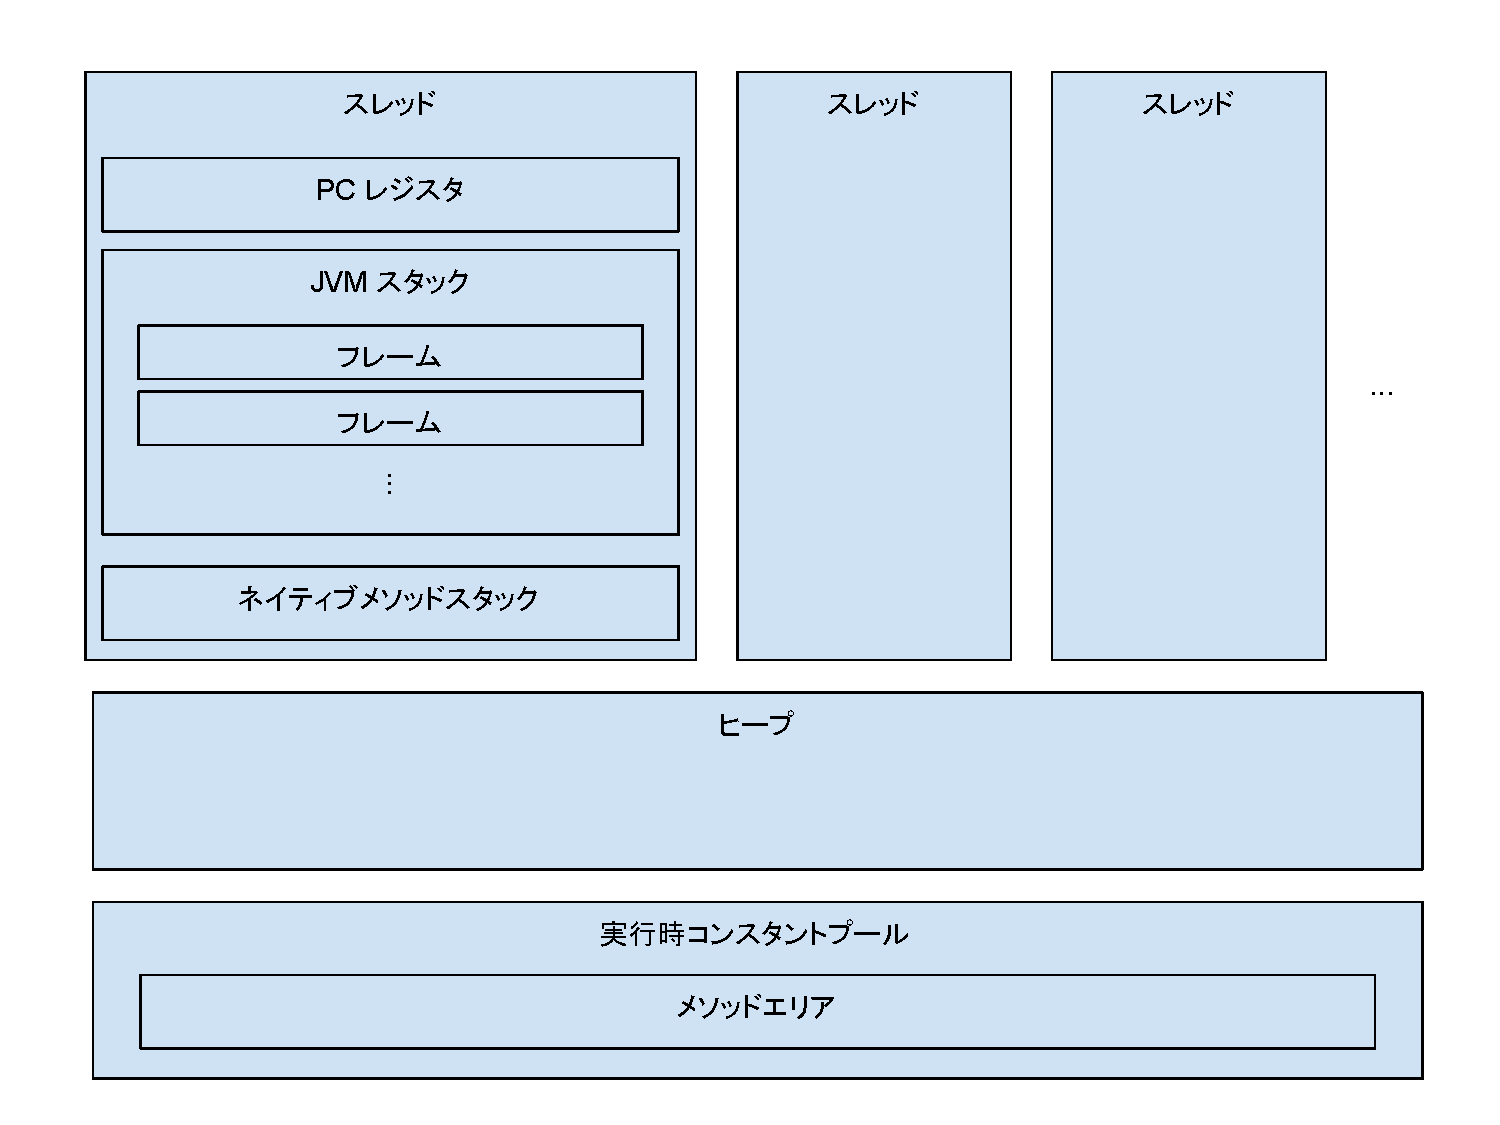
\includegraphics[bb=0 0 800 600,width=12cm]{img/jvm_architecture.pdf}
  \end{center}
\end{figure}

JVMのフレームについて、概観を\ref{fig:jvm_frame}に示す。

\begin{figure}[htbp]
  \caption{JVM構成概観}
  \label{fig:jvm_frame}
  \begin{center}
    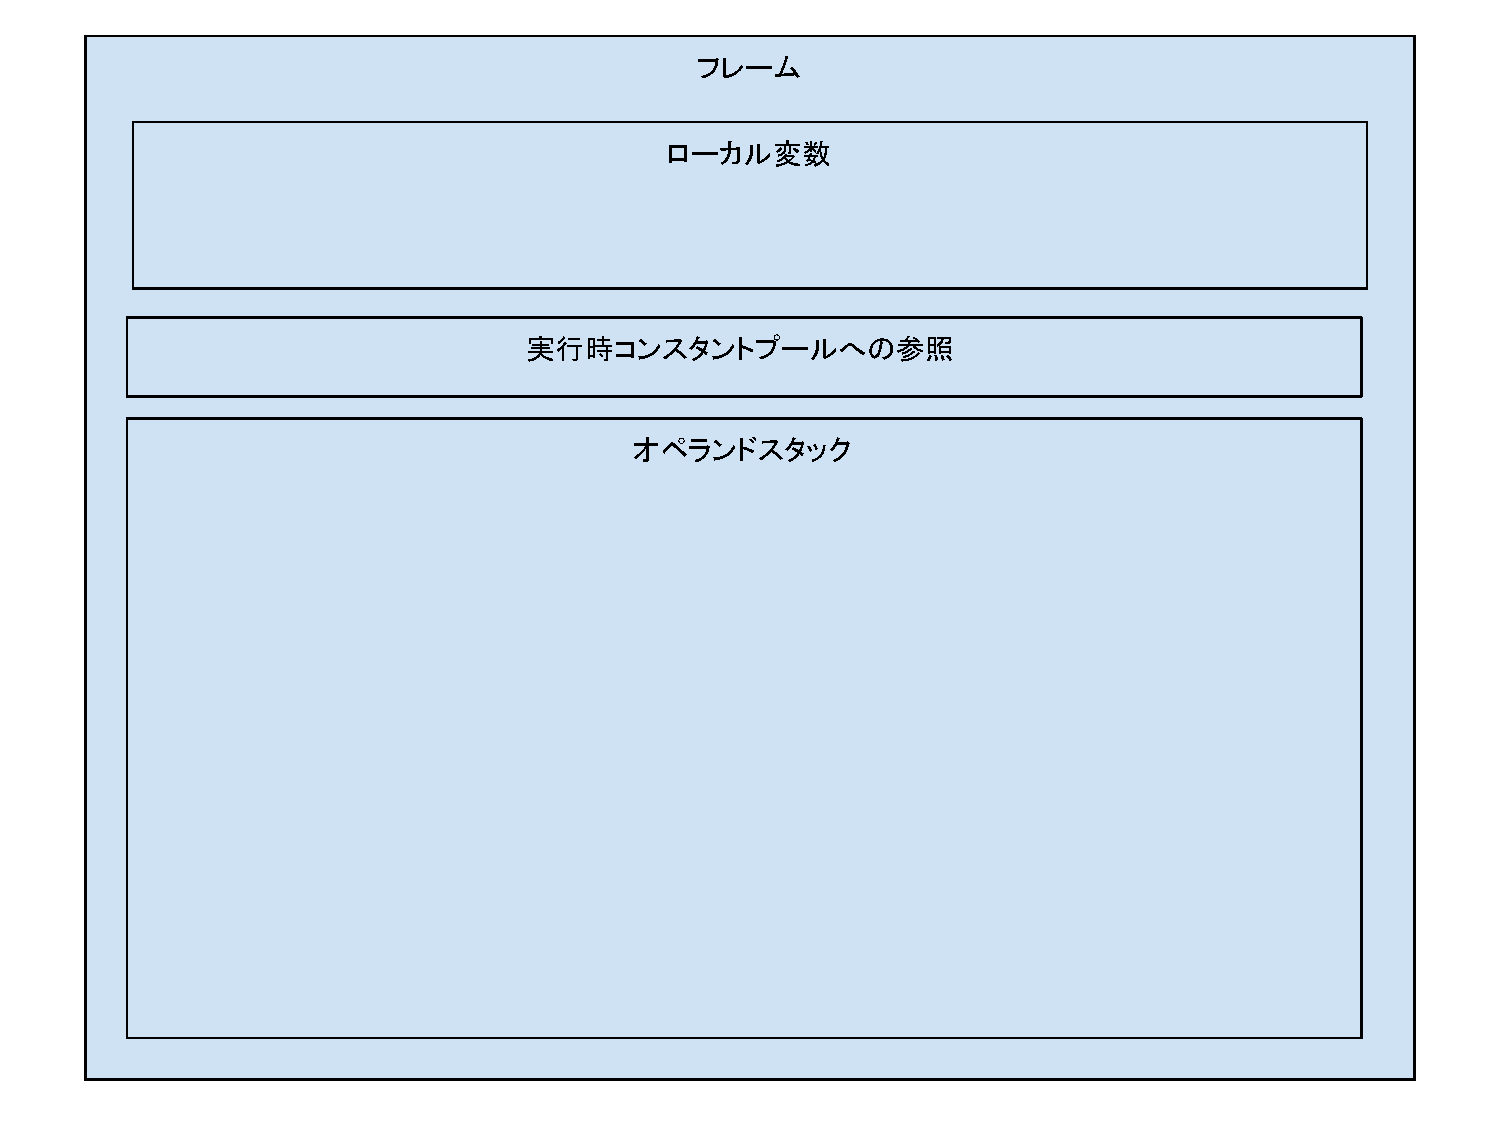
\includegraphics[bb=0 0 800 600,width=12cm]{img/jvm_frame.pdf}
  \end{center}
\end{figure}

\subsection{型}

JVMがサポートする型には、プリミティブ型と\verb|reference|型(参照型)の2種類がある。

プリミティブ型には、数値型と\verb|boolean|型、\verb|returnAddress|型が存在する。

数値型には、以下の7種類が存在する。なお、符号付きの整数は2の補数として表現され、浮動小数点数はIEEE754規格\cite{ieee754}で定められた数値と対応している。
\begin{itemize}
  \item 整数型
  \begin{itemize}
    \item \verb|byte| 符号付き8ビット整数
    \item \verb|short| 符号付き16ビット整数
    \item \verb|int| 符号付き32ビット整数
    \item \verb|long| 符号付き64ビット整数
    \item \verb|char| 符号なし16ビット整数
  \end{itemize}
  \item 浮動小数点数型
  \begin{itemize}
    \item \verb|float| 単精度32ビット形式
    \item \verb|double| 倍精度64ビット形式
  \end{itemize}
\end{itemize}

\verb|boolean|型は、値\verb|true|と\verb|false|をそれぞれ1と0で表したものである。
JVMは\verb|boolean|型の値に対する演算を直接はサポートしておらず、\verb|int|型に変換することで行われる。

\verb|returnAddress|型は、特定の命令へのポインタが値となり、ジャンプ先やリターン先を指定するために用いられる。

\verb|reference|型は、クラス型、インターフェース型、配列型の3種類がある。

\subsection{命令セット}

JVMの命令セットは205の命令を持つ。これらの命令について機能ごとに大別した上で、それぞれの数を表\ref{tb:jvm_opcodes}に示す。

\begin{table}[htbp]
  \caption{JVMが持つ命令セットの分類}
  \label{tb:jvm_opcodes}
  \begin{center}
    \begin{tabular}{|r|r|}
      \hline
      スタックへのロード、ストア & 86 \\ \hline
      スタックの操作(値の破棄、複製、スワップ) & 9 \\ \hline
      数値演算 & 37 \\ \hline
      比較 & 21 \\ \hline
      型の変換 & 15 \\ \hline
      オブジェクト、配列に対する操作、メソッドの呼び出し & 19 \\ \hline
      制御(\verb|goto|、\verb|return|など) & 13 \\ \hline
      同期処理(\verb|monitor|) & 2 \\ \hline
      例外 & 1 \\ \hline
      その他 & 5 \\ \hline
      \hline
      計 & 205 \\ \hline
    \end{tabular}
  \end{center}
\end{table}

なお、「その他」には、何もしない\verb|nop|、インデックスを2バイトで指定した上で特定の命令を実行する\verb|wide|、
そしてデバッグ用の\verb|breakpoint|、\verb|impdep1|、\verb|impdep2|が含まれる。

